\clearpage{}
\section{Define function testing. Explain the principles of cause-and-effect
graphs and their use in testing. Describe different types of performance
tests. Define and differentiate acceptance and installation testing.
Describe different types of acceptances tests. Describe and compare the
different types of test documents.}


\subsection{Function testing}

Does the integrated system perform as required by the requirements specification? 
\begin{itemize}

\item Ignores structure, focuses on functionality (black box). 
\item Follow functional requirement specifications subdivided in smaller
    units (in successive sets, on partial systems (spins)).
\end{itemize}

\subsection{Cause-and-effect graph}

Idea, deriving test cases from the requirements. Formalise the
requirements inputs/outputs. \newline

Make the cause-and-effect graph: Logical relationships between causes (inputs) and effects (outputs, transformations). Same idea as fault trees.

\begin{figure}[!ht]
    \centering
    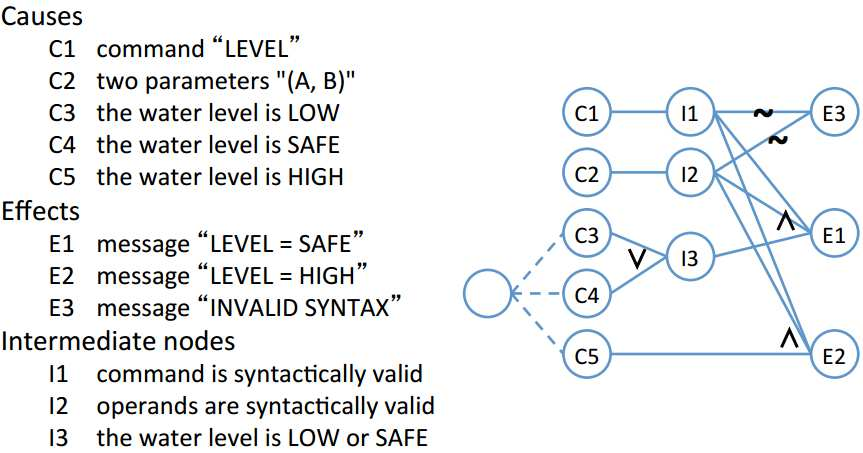
\includegraphics[width=0.7\linewidth]{causes_and_effects_graph.png}
\end{figure}

\begin{figure}[!ht]
    \centering
    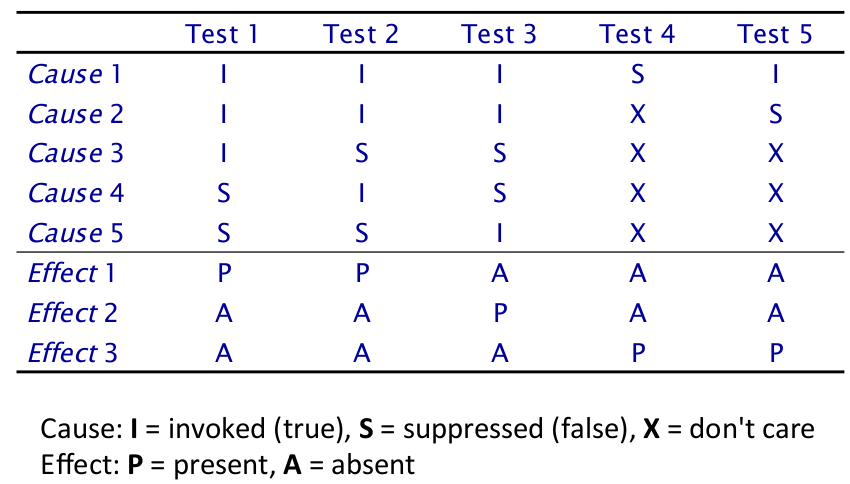
\includegraphics[width=0.7\linewidth]{decision_table.png}
\end{figure}

\subsection{Types of performance tests}
$\Rightarrow$ \textcolor{red!80!black}{Verify non functional requirements}

\begin{description}
    \item[Stress tests] max capacity for a short time
    \item[Volume tests] large amounts of data
    \item[Configuration tests] all possible configurations
    \item[Compatibility tests] interactions with other systems
    \item[Regression tests] performance is at least as good
    \item[Security tests] availability, confidentiality, integrity
    \item[Timing tests] response times
    \item[Environmental tests] physical factors: humidity, temperature, chocks, etc\ldots
    \item[Quality tests] reliability, maintainability, availability
    \item[Recovery tests] response to faults, loss of data, loss of power, etc\ldots
    \item[Maintenance tests] diagnostic tools and procedures
    \item[Documentation tests] available, consistent, easy to read, compliant
    \item[Human factors (usability) tests] ease of use, so/ware and documents
\end{description}

\subsection{Differences between acceptance and installation testing}

\begin{itemize}

    \item \textbf{Accepting testing}, goal: enable the customers and
        users to determine if the system meets their needs. Written,
        conducted and evaluated by the customers. If the customer
        approve then the product is accepted (wrt. The contract). 

        \paragraph{Types of acceptance tests}

        \begin{itemize}
            \item Benchmark test:
                Test case representing typical operation conditions to value competing products
            \item Pilot test:
                Test through real use but with guidance
            \item Alpha/beta test: For widely distributed products

                Alpha in house\newline
                Beta with selected pilot customer
            \item Parallel test:
                New system operates in parallel with old system
                E.g. Payroll system, you compare pay checks from old and new system

                Combine compatibility and function test
        \end{itemize}

    \item \textbf{Installation test}, at the user’s site, when configured, test if system works on site as in the lab.

        Test system completeness with element affected by the site
        conditions + regression tests (works on-site as in the lab)
\end{itemize}


\subsection{Types of test documents}

\begin{figure}[!ht]
    \centering
    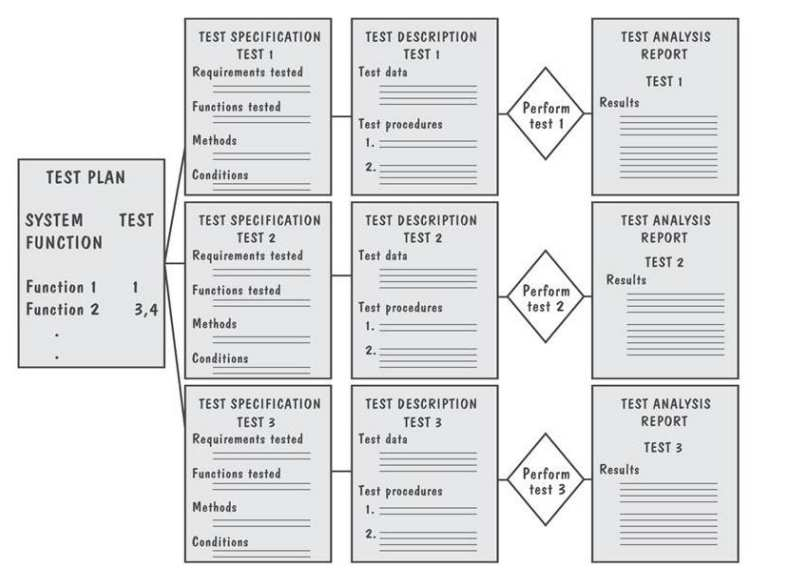
\includegraphics[width=\linewidth]{types_tests_document.png}
\end{figure}

\begin{description}
    \item[Test plan] describe the system and planned tests.
        \subitem{} Contains objectives, a summary, schedule etc\ldots
    \item[Test specification and evaluation] describe each test and evaluation of test results
        \subitem{} Specify requirements, test approach, completion criteria, evaluation methods, etc\ldots
    \item[Test description] test data and procedure (to realise it) for each test
        \subitem{} Specify means of control, the data (input output), the procedures (kind of script), etc\ldots
    \item[Test analysis report] result of each test
        \subitem{} Documents the results of a test, show how to determine completion, shows how to duplicate failure etc\ldots
\end{description}
